
% ════════════════════════════════════════════
% 数据理解与分布诊断（5.1）
% ════════════════════════════════════════════
\subsection{数据理解与分布诊断}

\subsubsection{数据口径与变量角色}

本部分不追求拟合模型，而是要把“数据能支持什么样的模型”说清楚。原始表共 500 行、8 个字段，一行即一条帖子，7 个输入变量加 1 个曝光结果；没有帖子编号与发布时间戳，同一主页只有一次观测，因此判定为帖子级截面数据，而不是面板或时间序列。按发帖前运营人员能否决定，帖子类型、内容主题、月份、星期、时段与付费标记属于发帖决策变量；粉丝规模由历史积累决定，属于账号状态变量；曝光总次数是发布后的结果。图\ref{fig:q1_dict}把变量的类型、取值类别与缺失状态集中呈现：X1 为连续变量但有 90 个重复取值，X2、X3 为名义变量，X4 至 X6 为周期性时间标记，X7 为二元指示变量且是唯一存在缺失的字段，Y1 为连续计数结果。计量单位上，X1 以人、Y1 以次计，X4、X5、X6 分别以月、星期与小时计；这些口径在后续所有模型中保持不变。

\begin{figure}[ht]
  \centering
  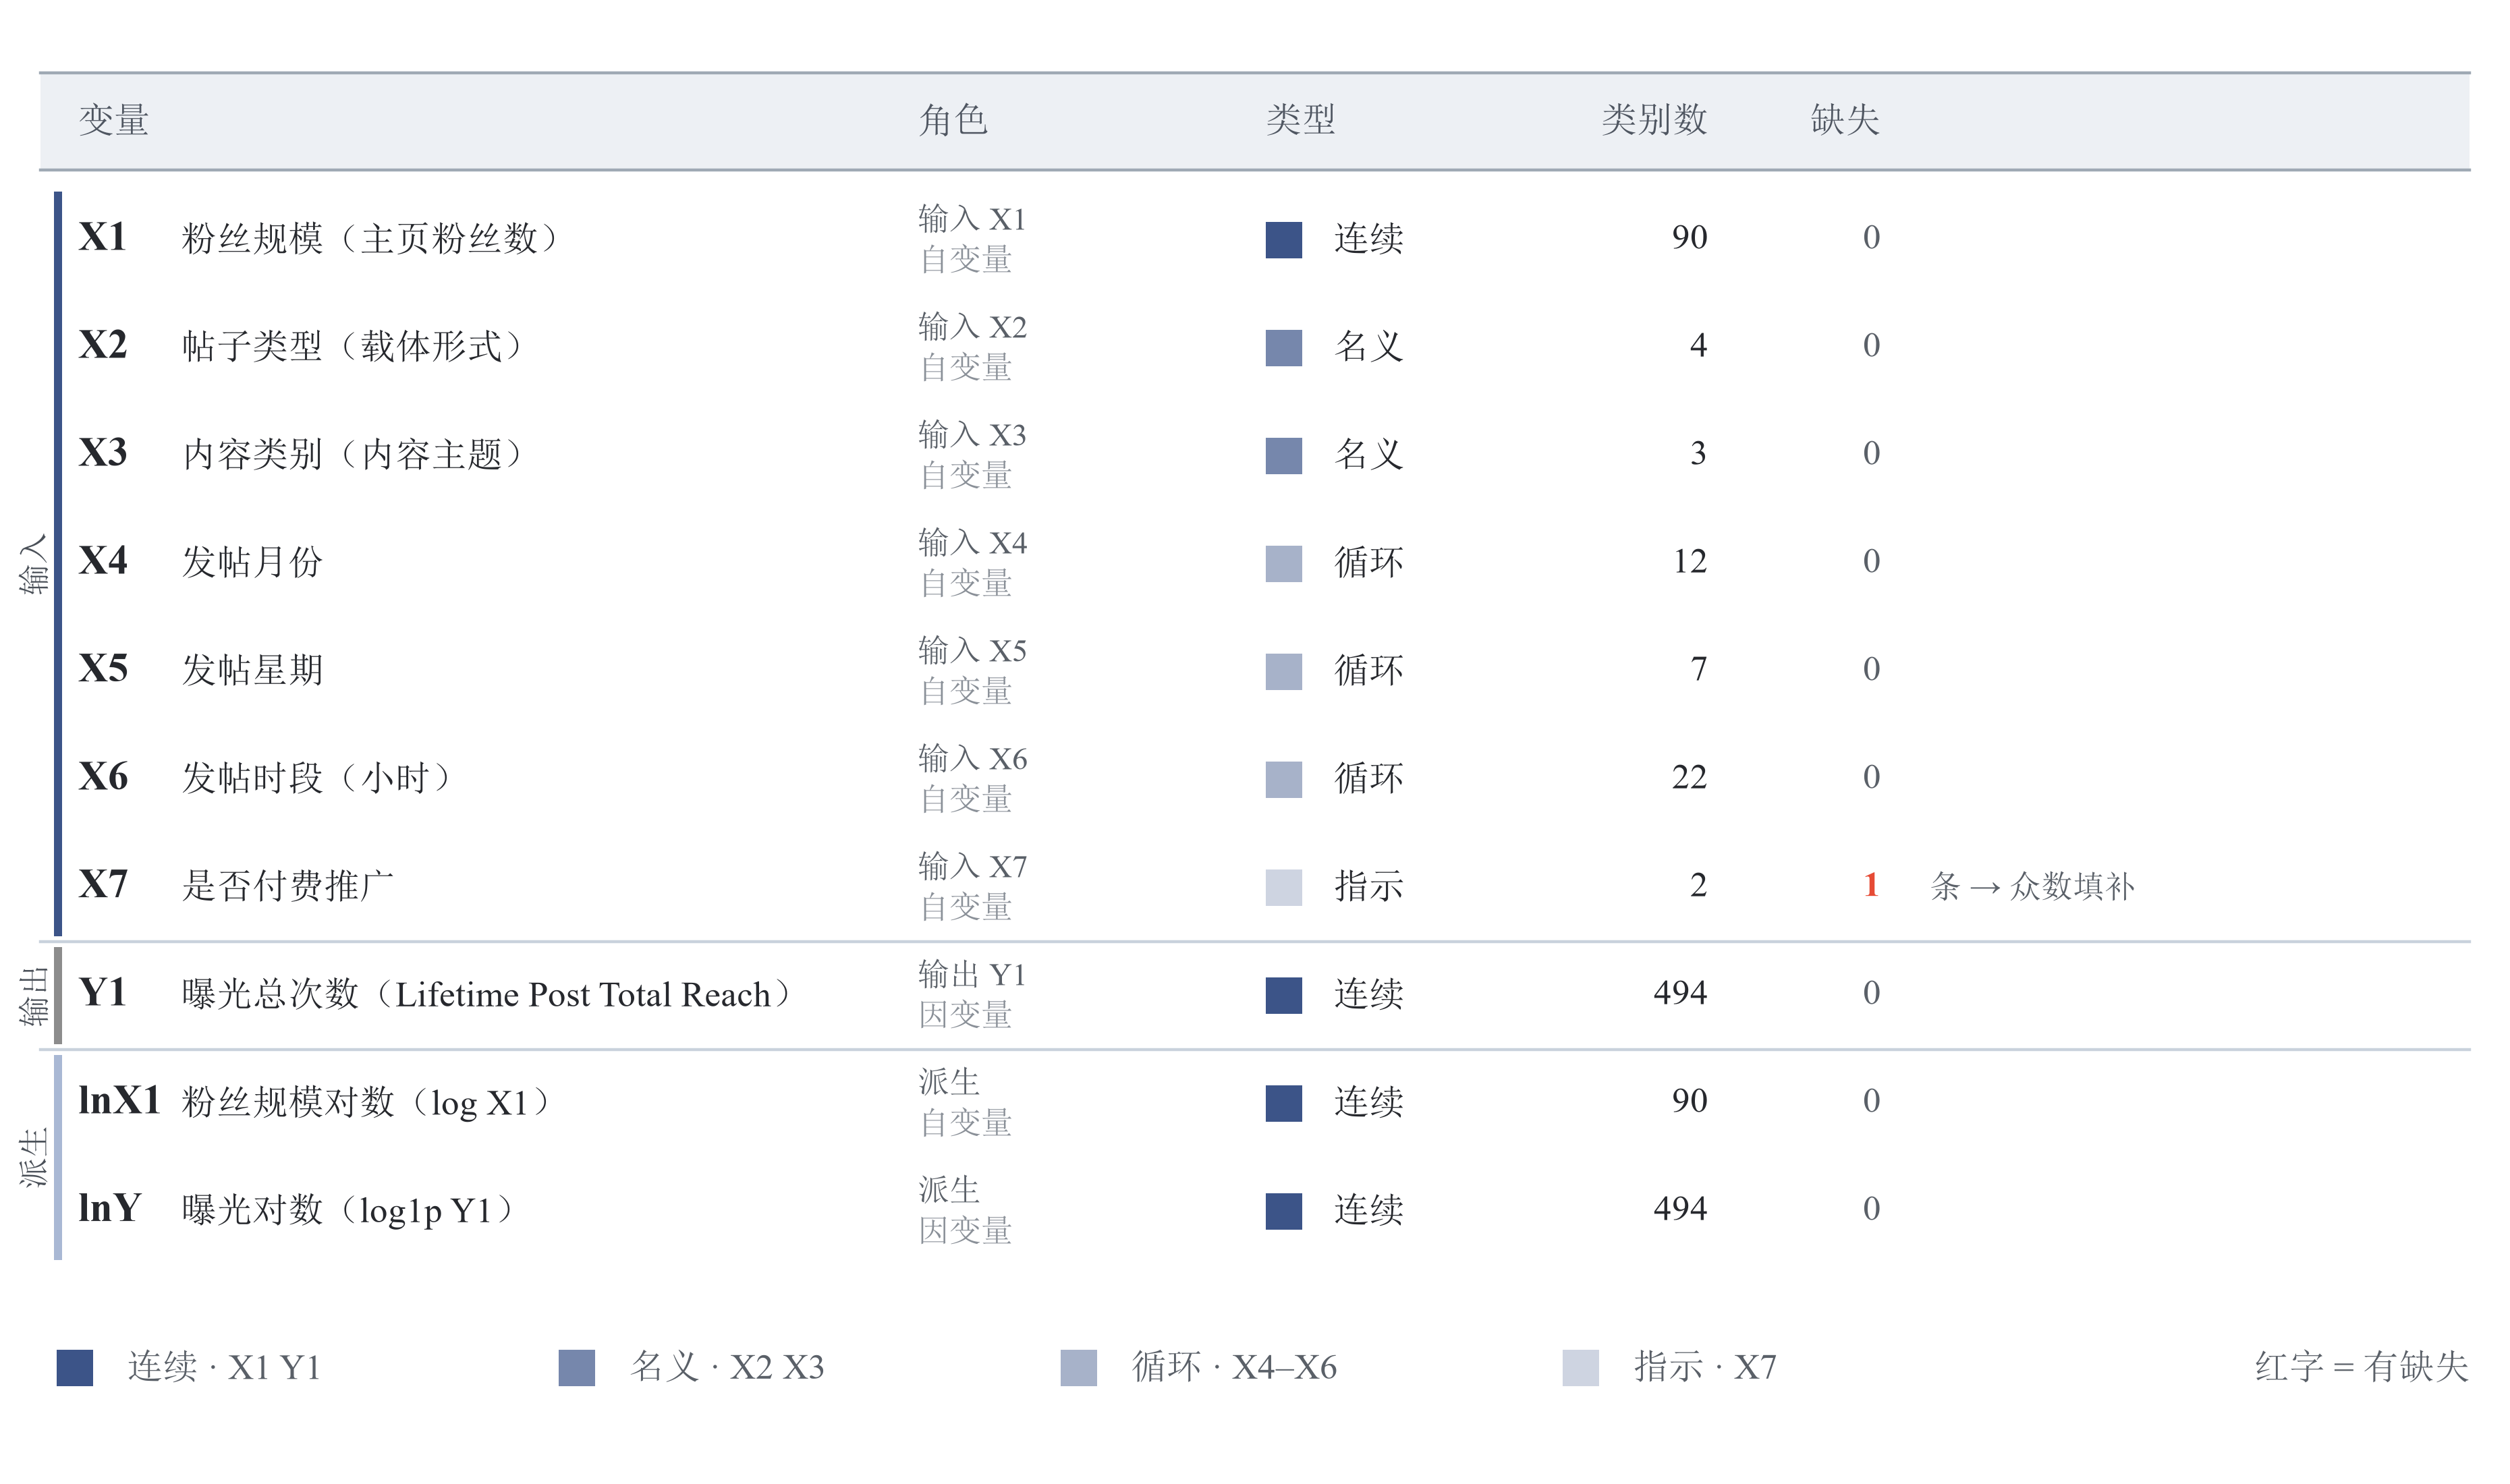
\includegraphics[width=0.68\textwidth]{../求解/问题一/结果/图14_变量字典与缺失.png}
  \caption{变量字典、类型与缺失状态}
  \label{fig:q1_dict}
\end{figure}

图\ref{fig:q1_dict}还显示，X1 只有 90 个不同取值，说明粉丝数按天或按批次更新，同一数值被多条帖子共享；X6 在样本中有 22 个取值，0 时与 21 时没有帖子；Y1 有 494 个不同取值，只有少数重复。上述结构决定了后续不能把 X1 当作独立的时间序列，也不能对 X6 逐小时生成哑变量。

\subsubsection{分布形态与共线证据}

曝光量呈典型的重尾右偏。表\ref{tab:q1_desc}显示，均值为 29,586 次，约为中位数 9,051 次的 3.27 倍；最大值 1,110,282 次为中位数的 122.67 倍；偏度 8.33、峰度 93.05，远超正态分布的参考范围。粉丝规模均值 123,194 人、标准差 16,273 人，最大值与最小值之比仅 1.71，量级跨度有限。付费帖子 139 条，占 499 条有效记录的 27.9\%，填补后占 500 条的 27.8\%。

图\ref{fig:q1_dist}把分布与分组差异放在同一画布。左上直方图在对数横轴上仍向右拖尾，中位数附近堆积了大量帖子，10 万次以上的极端帖子数量很少；右上雨云图显示，付费组的中位曝光为 12,060 次、自然组为 8,443 次（完整案例 $n=360$），中位数提升 42.8\%。下方按类型与主题分组的雨云图表明，视频组的中位数最高（56,950 次），状态组次之（20,849 次），图片组与链接组接近（8,132 与 9,773 次），三类主题的中位数分别为 10,417、8,962 与 8,303 次。分组差异为后续回归提供了初步线索，但未控制月份与内容构成，不能直接当作净效应。

\begin{figure}[p]
  \centering
  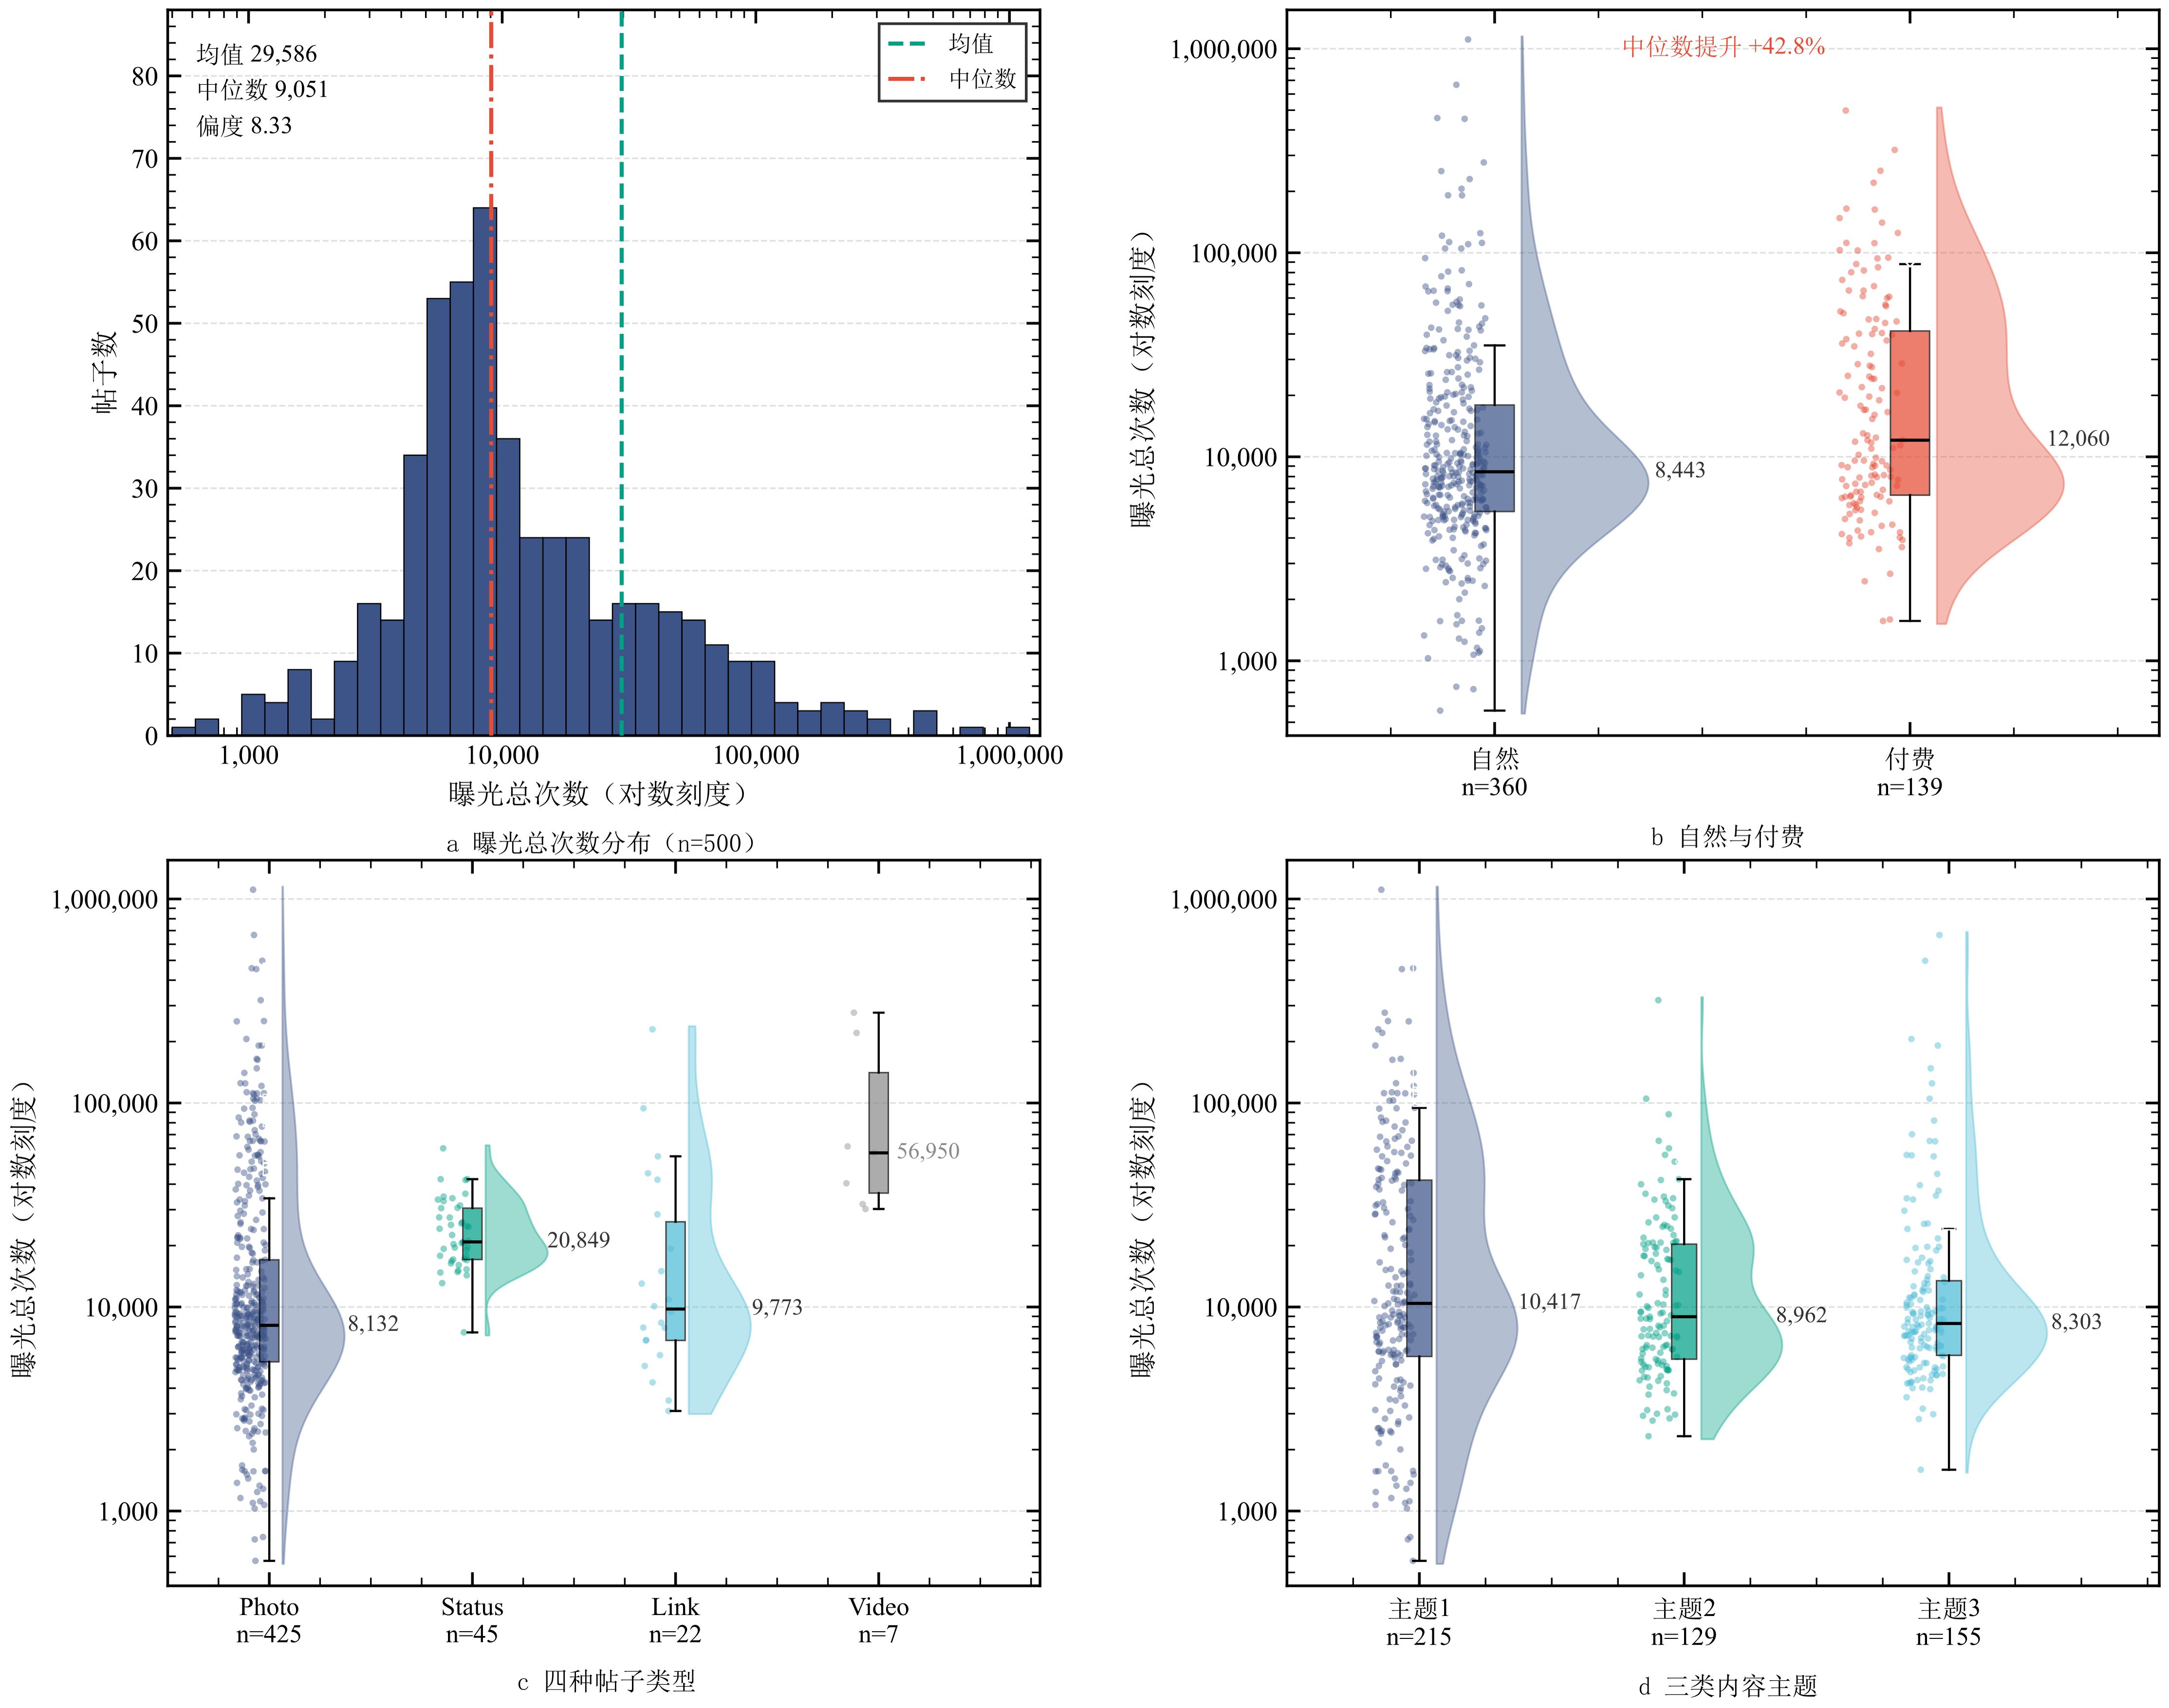
\includegraphics[width=0.66\textwidth]{../求解/问题一/结果/图1_曝光与分组分布.png}
  \caption{曝光量分布与分组差异}
  \label{fig:q1_dist}
\end{figure}

图\ref{fig:q1_structure}从构成、主题分布与联合分布三个角度补充样本结构。左上图以中线为界，左侧为自然帖、右侧为付费帖：Photo 在两组中都占 85\% 以上（自然 307 条、付费 119 条），Status 与 Link 合计不足 15\%，Video 只有 7 条且其中 4 条为付费，付费占比 57.1\%，说明类型效应主要由 Photo 与 Status 支撑，Video 的估计必然带有较大不确定性。右上图把三类主题的曝光分布、箱线与原始散点叠在一起，三组对数曝光的中位数分别为 9.25、9.09、9.02，主题 1 的分布整体略高，但三组重叠很大，单看主题不足以区分帖子表现。下方联合密度图的散点呈近竖直云团，粉丝规模对数与曝光对数的 Pearson 相关系数仅为 $-0.082$（$p=0.066$），上缘与右缘的边缘直方图进一步显示：两组在粉丝规模上几乎完全重合，而在曝光轴上付费组整体右移。由此可见，粉丝规模既不能单独解释曝光，也不足以区分付费与自然帖子，后续模型应把重点放在内容与投放变量上。

\begin{figure}[p]
  \centering
  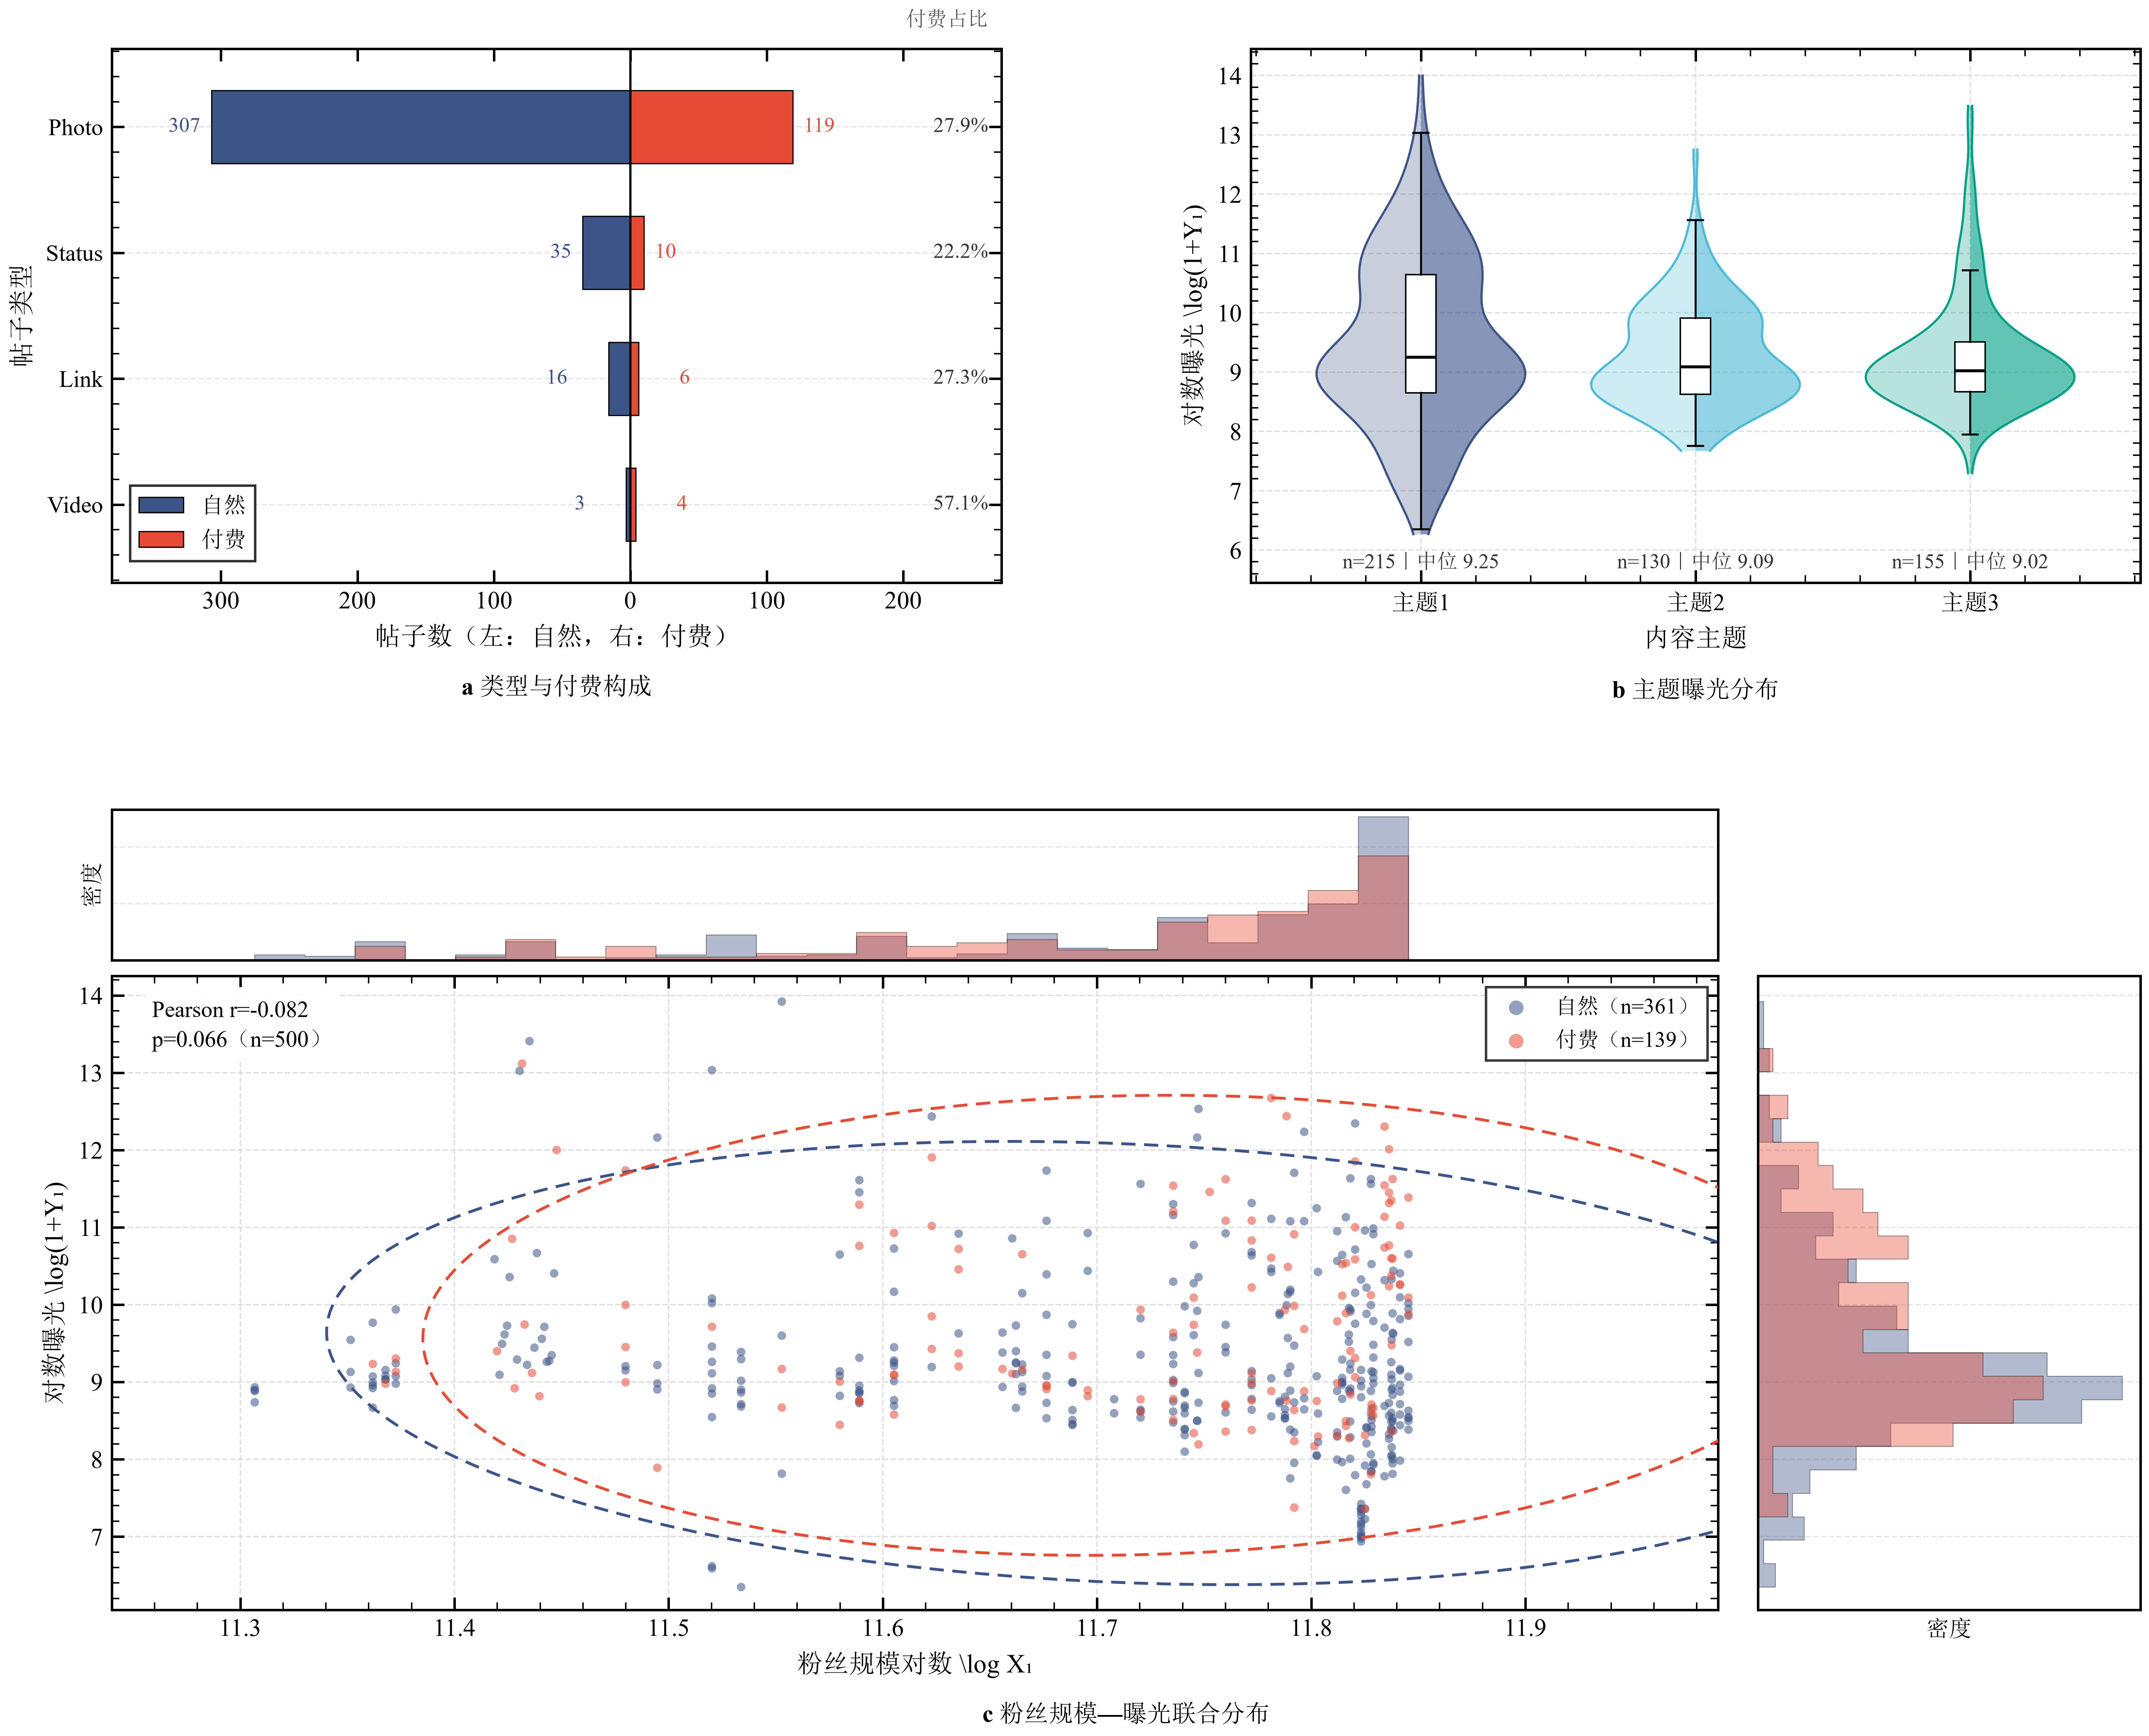
\includegraphics[width=0.66\textwidth]{../求解/临时产物/补充图1_样本结构.png}
  \caption{样本构成、主题分布与粉丝—曝光联合分布}
  \label{fig:q1_structure}
\end{figure}

表\ref{tab:q1_desc}同时给出共线证据。粉丝规模与月份的 Pearson 相关为 0.941、Spearman 相关为 0.996；以月份哑变量对粉丝规模对数做辅助回归，解释度达 0.9917，月内标准差仅 0.0130，月内方差占比仅 0.83\%。按预设的三项判别标准，粉丝规模与月份属于同一变异维度，同时进入回归会使系数依赖极少量月内变异。这一结构在散点与月均值折线上表现为阶梯式上升：月均值几乎单调递增，同一月份内部的粉丝规模对数只在极小范围内波动，偏差幅度远小于月间差异。这意味着粉丝规模在本样本中更接近“时间标签”而非独立解释变量。

\begin{figure}[htbp]
  \centering
  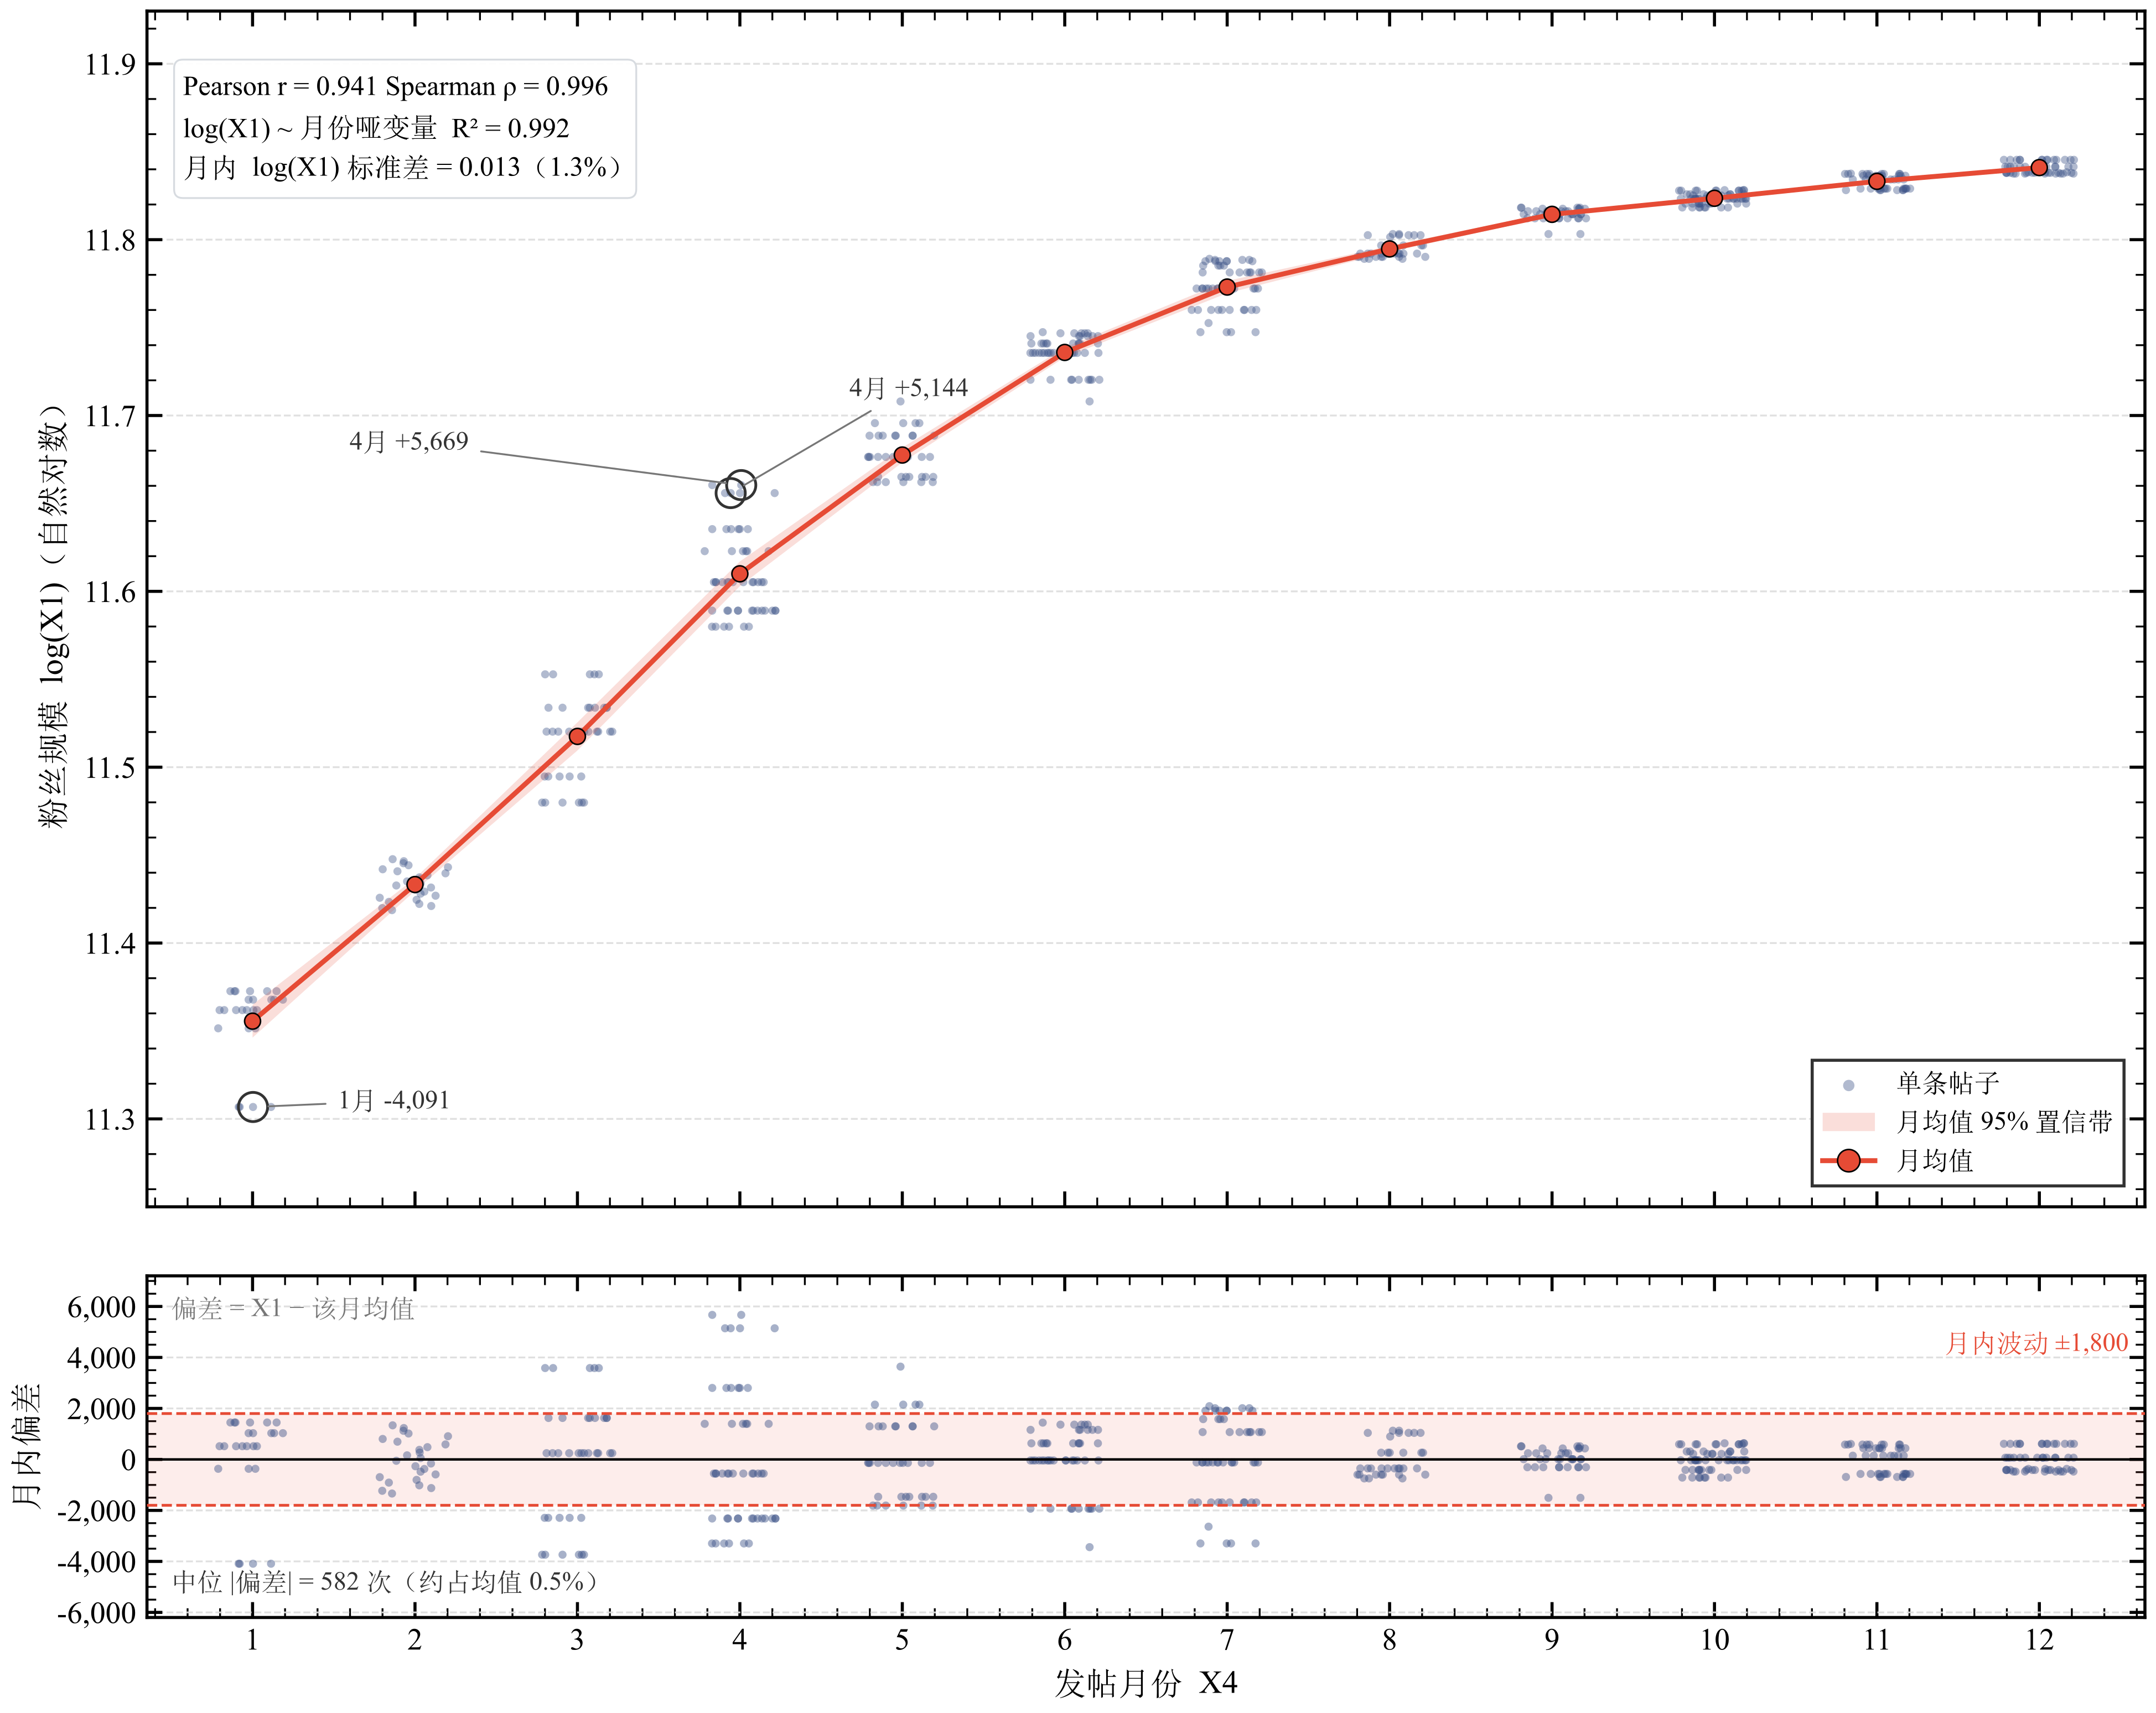
\includegraphics[width=0.74\textwidth]{../求解/问题一/结果/图2_粉丝规模与月份共线.png}
  \caption{粉丝规模与月份的共线结构：月度阶梯与月内偏差}
  \label{fig:q1_collinear}
\end{figure}

图\ref{fig:q1_collinear}把这一结构直接画了出来：主图按月排列的散点几乎落在同一条单调上升的曲线上，红色折线为月均值、浅红带为 95\% 置信带，圈注点为月内偏差最大的三条帖子；下挂小图给出每条帖子相对当月均值的偏差，绝大多数落在 $\pm 1{,}800$ 次以内，中位绝对偏差仅 582 次，与月间上万次的落差形成鲜明对比。

相关分析进一步给出主要变量的 Spearman 相关矩阵。曝光量与付费的相关系数为 0.171，是矩阵中与曝光关系最强的一项；与粉丝规模、月份的相关系数均为 $-0.135$，与内容主题为 $-0.080$，方向虽为负但幅度都很小；粉丝规模与月份的相关系数为 0.996，是矩阵中最突出的一格，说明二者几乎携带同一信息。相关矩阵只反映两两关系，且不包含帖子类型与发布时段，仍需回归控制其他变量后才能判断净效应。

\begin{figure}[htbp]
  \centering
  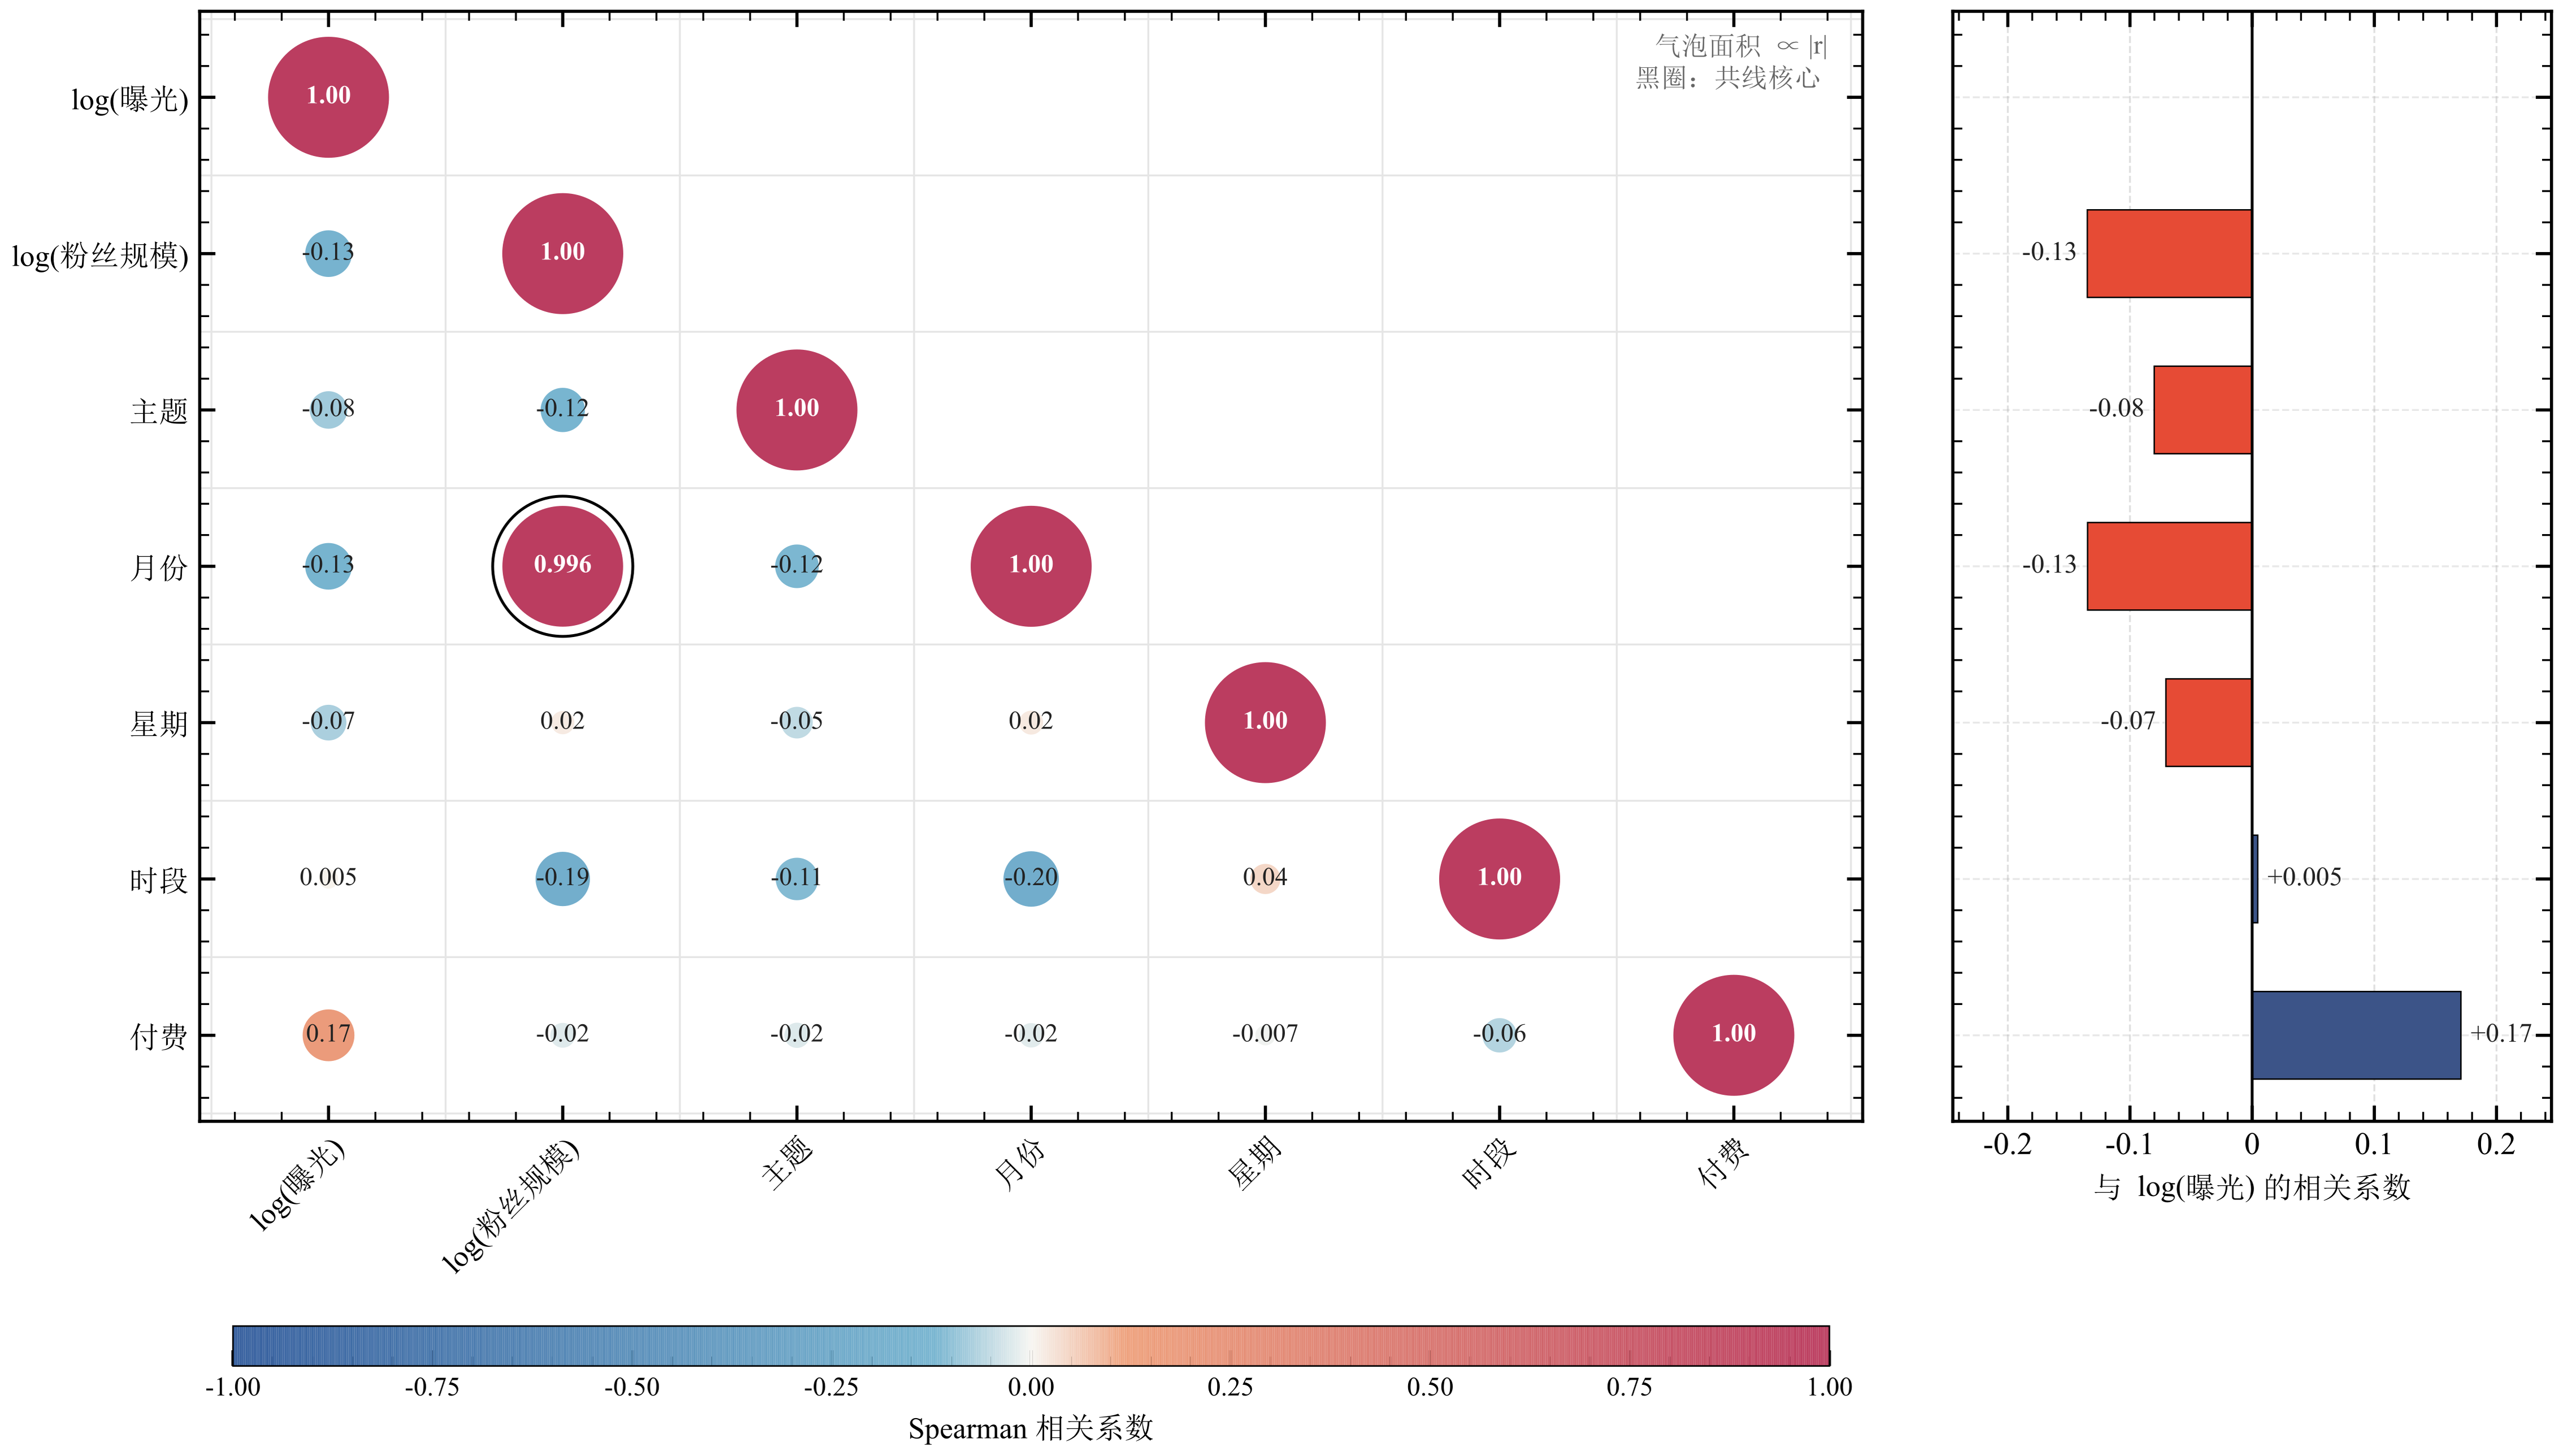
\includegraphics[width=0.82\textwidth]{../求解/问题一/结果/图3_相关系数热力图.png}
  \caption{变量间的 Spearman 相关矩阵与各变量对曝光的相关强度}
  \label{fig:q1_corr}
\end{figure}

图\ref{fig:q1_corr}的下三角气泡矩阵给出同一结论：除粉丝规模与月份那一格（黑圈标注，$r=0.996$）外，其余相关系数绝对值都不超过 0.20；右侧条形把各变量与曝光的相关系数单独列出，均为弱相关，说明单一变量都不足以解释曝光差异。


\begin{longtable}{>{\centering\arraybackslash}p{0.40\textwidth}>{\centering\arraybackslash}p{0.20\textwidth}>{\centering\arraybackslash}p{0.32\textwidth}}
  \caption{样本结构与共线指标}
  \label{tab:q1_desc} \\
  \toprule
  指标 & 数值 & 说明 \\
  \midrule
  \endfirsthead
  \caption{样本结构与共线指标（续）} \\
  \toprule
  指标 & 数值 & 说明 \\
  \midrule
  \endhead
  \bottomrule
  \endfoot
  样本量 & 500 & 每条记录对应一条帖子 \\
  变量数 & 8 & 7 个输入加 1 个输出 \\
  X1 唯一值数 & 90 & 同一粉丝数被多条帖子共享 \\
  X7 缺失数 & 1 & 占 0.2\%，仅第 499 行缺失 \\
  Y1 均值/中位/最大 & 29,586/9,051/1,110,282 & 最大值约为中位数的 122.67 倍 \\
  Y1 偏度/峰度 & 8.326/93.053 & 右偏、厚尾 \\
  log1p(Y1) 偏度/峰度 & 0.734/0.821 & 变换后接近对称 \\
  Pearson $r(X_1,X_4)$ & 0.941 & 线性同步程度高 \\
  Spearman $\rho(X_1,X_4)$ & 0.996 & 单调同步程度极高 \\
  $R^2(\log X_1\sim\text{月份})$ & 0.9917 & 99.17\% 的变异在月间 \\
  月内方差占比 & 0.0083 & 月内仅剩 0.83\% 的信息 \\
\end{longtable}

综合以上结果，数据理解的核心结论不是“粉丝规模影响曝光”，而是“粉丝规模与月份共同刻画了账号成长的时间维度，二者不能同时识别”。这一结论直接决定了后续的建模策略：以月份固定效应吸收规模趋势，把粉丝规模留作稳健性对照，而不是强行解释其系数。
